\documentclass[11pt,a4paper]{scrartcl}

\usepackage[ngerman]{babel}
\usepackage[latin1]{inputenc}
\usepackage{graphicx}
\usepackage{rotating}

\usepackage{amsmath}
\usepackage{amsfonts}
\usepackage{amsthm}
\usepackage{mathtools}

\usepackage{listings}
\usepackage{color}




\begin{document}

\pagestyle{plain}
\pagenumbering{arabic}


\section*{Example 1: Bedingungsfortpflanzung}

Das Verfahren der Bedingungsfortpflanzung pr�ft die Widerspruchsfreiheit der im Problem vorhandenen Bedingungen, um die neuen Bedingungen ableiten zu k�nnen (eng. {\bf arc consistency checking}).

Hier geht man davon aus, dass die Bedingungen zwischen der Variablen eines CSP immer nur zwei Variablen beeinflussen. In diesem Fall kann CSP als ein Bedingungsgraph dargestellt werden. Variablen des CSP bilden die Menge der Knoten des Graphen. Die Knoten sind adjazent, wenn es eine Bedingung gibt, die die entsprechende Variable verbindet.

Sei eine Bedingung $C_{ij}$ zwischen den Variablen $x_i$ und $x_j$ gegeben. Der Bogen $(x_i,x_j)$ hei�t widerspruchsfrei (eng. {\bf consistent}), wenn f�r jeden Wert $a\in D_i$ ein Wert $b\in D_j$ existiert, sodass die Zuweisungen $x_i=a$ und $x_j=b$ die Bedingung $C_{ij}$ erf�llen.

\begin{figure}[h]
	\vspace{-10pt}
	\vbox{
		\centering
		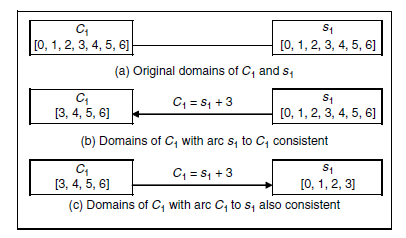
\includegraphics[scale=0.7]{../fig/ConstraintPropagation1.png}
	}
	\caption{Reduktion des Suchraums mithilfe der Widerspruchsfreiheit eines Bogens}
	\label{fig:ConstraintPropagation1}
\end{figure}

Alle Werte $a\in D_i$, f�r die dies nicht gilt, k�nnen aus dem Definitionsbereich $D_i$ der Variable $x_i$ gel�scht werden, da sie keine zul�ssige L�sung bilden k�nnen. Das L�schen von solchen Werten macht den Bogen widerspruchsfrei. Ein einfaches Beispiel der Bogenwiderspruchsfreiheit ist auf der Abbildung \ref{fig:ConstraintPropagation1} dargestellt.

\begin{figure}[htb]
	\centering
	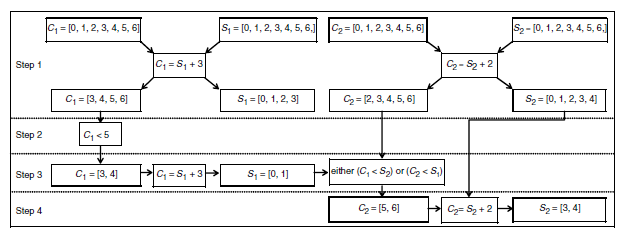
\includegraphics[scale=0.8]{../fig/ConstraintPropagation2.png}
	\caption{Reduktion des Suchraums mithilfe der Widerspruchsfreiheit mehreren Bogen}
	\label{fig:ConstraintPropagation2}
\end{figure}

Offensichtlich ist, wenn alle Bogen widerspruchsfrei gemacht wurden, ist der Suchraum des Problems kleiner geworden (engl. {\bf domain reduction}). Nach der Reduktion des Suchraums soll das Suchen nach der L�sung einfacher werden.

Zu bemerken ist, dass die Bedingungsfortpflanzung die Information der Definitionsbereiche der Variablen nicht nur innerhalb einer Bedingung benutzen kann, sondern auch zwischen mehreren Bedingungen. Dazu das Beispiel auf der Abbildung \ref{fig:ConstraintPropagation2}. Das f�hrt zu der so genannten Reduktion des Suchraums zwischen den Bedingungen (eng. {\bf between-constraint domain reduction}).





\end{document}

